\documentclass[twocolumn,10pt]{article}
\usepackage[a4paper, top=1.0in, bottom=1.0in, left=0.85in, right=0.85in]{geometry}

\usepackage{graphicx}
\usepackage{algorithm}  
\usepackage{algorithmicx}  
\usepackage{algpseudocode}  
\usepackage{amsmath}
\usepackage{url}

\renewcommand{\algorithmicrequire}{\textbf{Input:}}  
\renewcommand{\algorithmicensure}{\textbf{Output:}}  
\graphicspath{{figure/}}

\begin{document}

\date{November 17th, 2016}

\title{\bf Grouper: A Group Finance Manager on Mobile Devices Using Untrusted Servers}

\author{
	Meng Li, 201620728  
	\\ Supervisor: Yasushi Shinjo
}

\maketitle

\section{Introduction}
Conventional mobile applications are built based on a client-server mode. This requires central servers for storing shared data. The users of such mobile applications must fully trust the central server and their application providers. If a central server is compromised by hackers, user information may be revealed because data is often stored on the server in cleartext. Users may lose their data when service providers shut down their services. 

A popular approach to address the central server problem is using P2P(Peer to Peer) to transfer user data between devices. However, there is an obvious problem in such a P2P approach. Data transfer can only be finished during two devices are online at the same time. Another problem is that the number of P2P connections becomes large  fast as the number of users increases. 

We are implementing a mobile application that is not relied on trusted central servers. Concretely, we are developing a group finance manager application. We call it Grouper. Unlike P2P systems, we use multiple untrusted servers for data transfer. Data is divided into several pieces and uploaded to diverse servers. Each server can only keep a piece of data temporarily. A piece will be deleted after a period of time. Those two methods ensure that user data cannot be cracked easily. In addition, all devices of group members keep a complete data set, and data can be recovered even untrusted servers shut down.

\section{Design}

We design a group finance manager application, Grouper, on mobile devices. This does not rely on trusted central servers. 

\subsection{Group Finance Manager}
 In Grouper, group members generate records about amounts of money, classifications, accounts, shops, remarks and times in their devices. For example, Alice records that she ate breakfast (classification) in the center canteen (shop) at 8:00 AM (time) on November 1st, 2016, and she paid her breakfast by her credit card (account). These items are created by users as they want. They can choose an item from existing ones when they want to add new records.

 With data synchronization, group members can also share their records with other group members. Therefore, group income and expenditure information are analyzed and shown to all members. Grouper uses multiple untrusted servers to synchronize and avoids relying on trusted central servers. To create a group in Grouper, the owner of this group needs to register and set access keys in untrusted servers. The owner passes the access keys to group members by a face-to-face way.

\subsection{Shamir's Secret Sharing}
In Grouper, secret sharing plays an indispensable role in protecting user data from getting lost or destroyed. In a secret sharing scheme, a dealer securely shares a secret with a group of members by generating $n$ shares using a cryptographic function\cite{smith2013layered}. At least $k$ or more shares can reconstruct the secret, but $k-1$ or fewer shares can obtain nothing about the secret\cite{pang2005new}. We describe this scheme as a function $f(k, n)$, where $n$ is the number of all shares, and $k$ is the threshold to combine shares.  We use Shamir's secret sharing that  is a popular technique to implement threshold schemes.

\subsection{Data Synchronization Using Multiple Untrusted Servers}

We design Grouper based on data synchronization through multiple untrusted servers rather than a single server. There are three principles in our proposal. 

Firstly, a server transfers data as similar to a router, but does not keep it permanently. Most current popular client-server applications store their user data on several central servers, and the user's data will not be deleted unless the user deletes his account. Grouper uses untrusted servers as a bridge for transferring data. Consider that a group includes three members: Alice, Bob and Carol. Alice creates a new record in her device, this record is uploaded to untrusted servers, and the record on servers will be deleted after Bob and Carol download it from servers.

Secondly, a server keeps data temporarily. We define a period of time in which data can be kept in a server. In this paper, we set this period to 1 hour for our example situations. The record Alice uploaded to untrusted servers can exist for 1 hour. After 1 hour since uploaded, this record will be deleted. Alice requires to upload this record again to serves until all of other members have downloaded successfully. The longer keeping period means the higher risk of data reveal. We will find suitable periods as the number of group members, security requirement and others. 

Thirdly, servers do not know the cleartext of data. Keeping data temporarily cannot ensure data security, because servers know the cleartext of data in this temporary period. For this problem, developers often encrypt data before uploading to servers, and this needs a decryption key to decrypt data in other devices. In order to distribute the decryption key, users should share it by themselves. In Grouper, we do not encrypt data but we use a secret sharing scheme as described in Section 2.2. Servers do not know the cleartext of a share generated by a secret sharing scheme.

\begin{figure}[t]
\centering
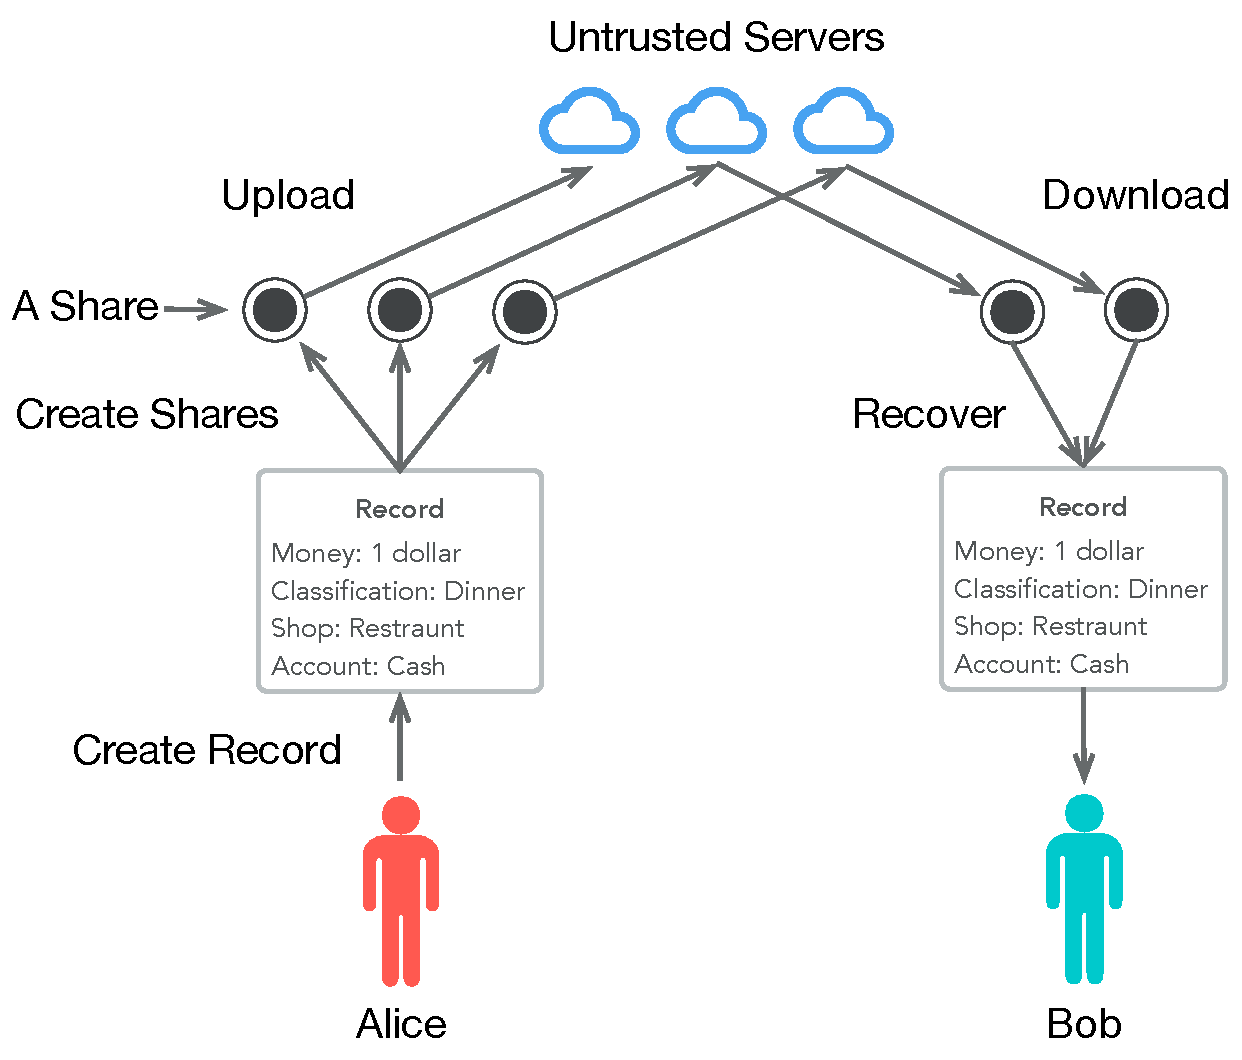
\includegraphics[scale=0.38]{sync_flow}
\caption{Flow of synchronization.}
\end{figure}

Figure 1 describes our synchronization flow based on these three principles. At first, Alice adds a record and Grouper creates three shares by a secret sharing scheme where $n$ is three and $k$ is two. Next, Grouper uploads those shares to three untrusted servers. When Bob is online, Grouper in Bob's device downloads two shares from servers and recovers the new record created by Alice. In this situation, Grouper can recover the record after getting two or more shares. In this process, each server is separated from other servers, and cannot access to other servers. This means these servers cannot recover user data because they do not have permission to access other untrusted servers. In our proposal, only group members have permission to access these untrusted servers.

\subsection{Reliable Synchronization}
Grouper should provide a reliable synchronization service. For example, Alice is a user in a group and creates a new record in her device. All of other members in a group should synchronize this record, even if this record may be deleted by untrusted servers after a period of time. We call this problem \emph{reliable synchronization}.

Figure 2 describes an unreliable situation that data cannot be synchronized. Alice sends a new record to untrusted servers at 10:00 AM and Bob downloads it successfully at 10:30 AM. Carol becomes online at 11.30 AM and fails to download shares of this record because they have been deleted by servers. To solve this problem, Alice should upload her new record again until Carol downloads it successfully. However, it is hard for Alice to get the information that all of other members in her group have downloaded. We must find an efficient way for notifying Alice that all members have synchronized successfully.

\begin{figure}[t]
	\centering
	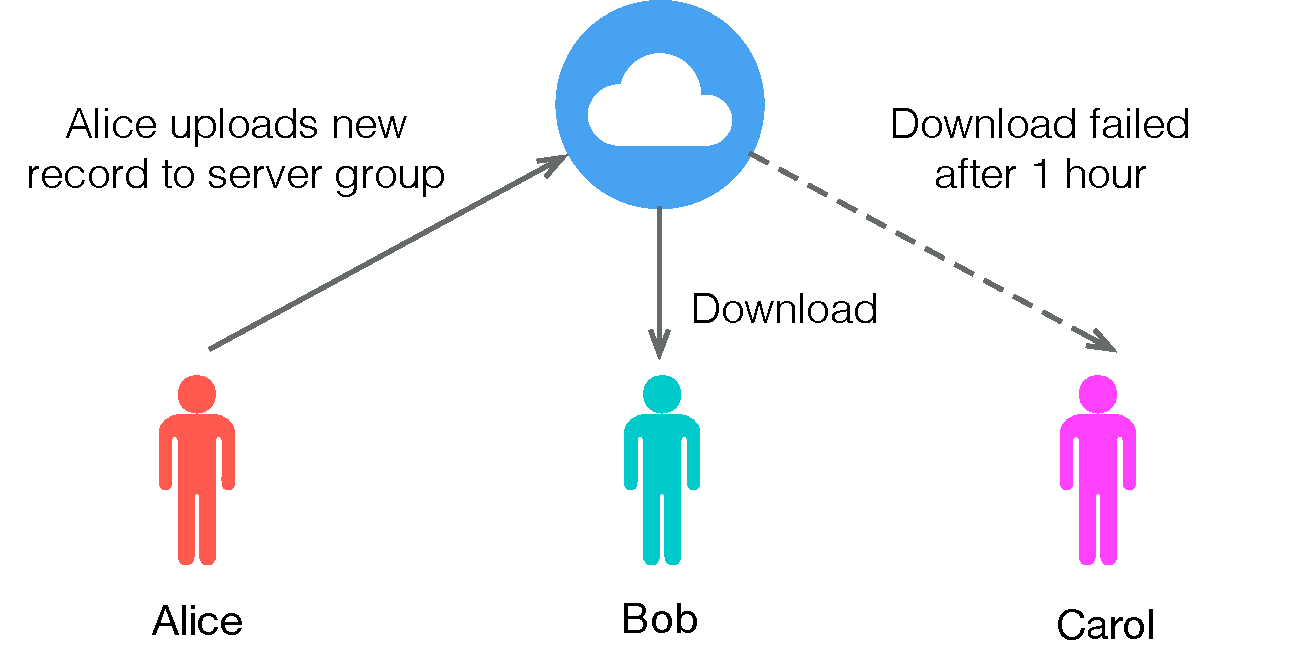
\includegraphics[scale=0.38]{unreliabe_sync}
	\caption{Unreliable synchronization.}
\end{figure}

We must consider a further problem that Carol, who is offline, can attack this group by being lazy. Alice, the record creator, has to upload shares to untrusted servers indefinitely. We are addressing this problem by holding a list group members in untrusted servers.

\subsection{Creating a Group}

A group in Grouper is created by its owner. For example, Alice is a group owner and she registers her group in multiple untrusted servers by submitting her user information, group ID and group name. Here, the group ID and group name are assigned by Alice and they should be same in all untrusted servers of this group. In each untrusted server, its Web service creates this new group successfully and returns a master key including the highest privilege for Alice.

Figure 3 shows the procedure to add a new member to a group. At first, when Bob wants to join Alice's group, he meets Alice by a face-to-face way. After establishing a connection between Alice's and Bob's devices, Bob's device sends his user information to Alice's device at first. Alice creates a new user called Bob in the three untrusted servers of her group. These servers return three access keys for Bob to Alice. At last, Alice sends these access keys and user information to Bob, so that he can access those untrusted servers.

\begin{figure}[t]
	\centering
	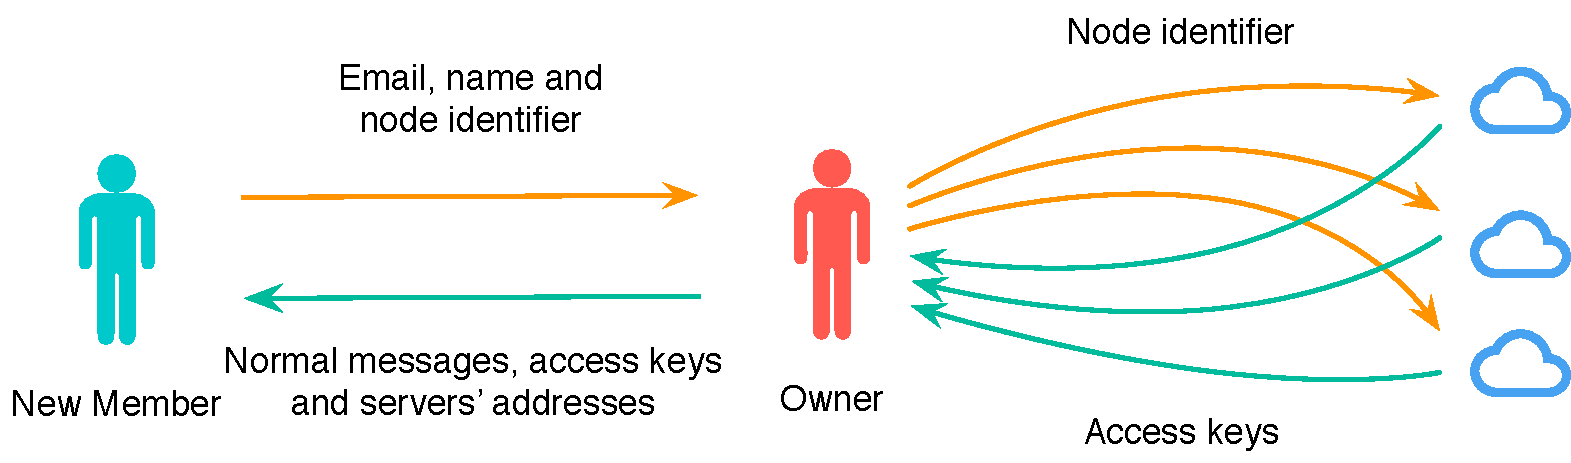
\includegraphics[scale=0.38]{add_member}
	\caption{Adding a new member.}
\end{figure}

\section{Implementation}
Grouper consists of clients that run an iOS application and multiple untrusted servers that run a Web service. In Section 2, we have introduced how to share strings with other deices via multiple untrusted servers. In this section, we describe persistent store and data synchronization. Grouper stores all data on mobile devices with an object-oriented way.

\subsection{iOS Application}
 Grouper uses Core Data\cite{coredata}, a native iOS framework to manage the model layer objects. Core Data provides generalized and automated solutions to common tasks associated with object life cycle and object graph management, including persistence. Sync\cite{sync} is a modern JSON synchronization framework for Core Data, and performs data synchronization by generating and parsing JSON strings. With Sync based on Core Data, we can concentrate on sharing with untrusted servers rather than data storage and synchronization.

In this paper, we use c-SSS\cite{c-sss}, an implementation of Shamir's secret sharing in the C language. This implementation supports the UTF-8 character set without limitation of length. It provides two main functions: \emph{generate}, which generates $n$ shares by a string text with the threshold $k$, and \emph{extract}, which recreates the text string from more than $k$ shares. 

c-SSS generates shares from a JSON string. There shares are stored as an entity in Core Data. Grouper generates shares and upload them by a REST API to servers.

Figure 4 describes the architecture of the iOS application running on clients. Grouper stores all data on mobile devices in an object-oriented way. Grouper uses Core Data to store and operate data as objects. \emph{NSManagedObject+HYPPropertyMapper} is a part of the Sync framework and creates JSON string from objects. The REST API provided by the Web service in untrusted servers uploads and downloads shares between clients and servers. User information and server information are transferred between clients using the Multipeer Connectivity framework.

Figure 5 is a screen shoot of the view \emph{Add Record}. In this view, users add a new record including amount of money, classification, account, a shop, time and remark in this view.

\begin{figure}[t]
	\centering
	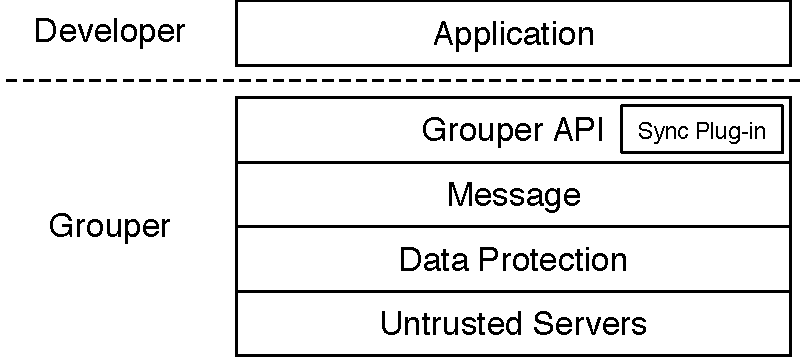
\includegraphics[scale=0.35]{architecture}
	\caption{Architecture of the iOS application.}
\end{figure}

\begin{figure}[t]
	\centering
	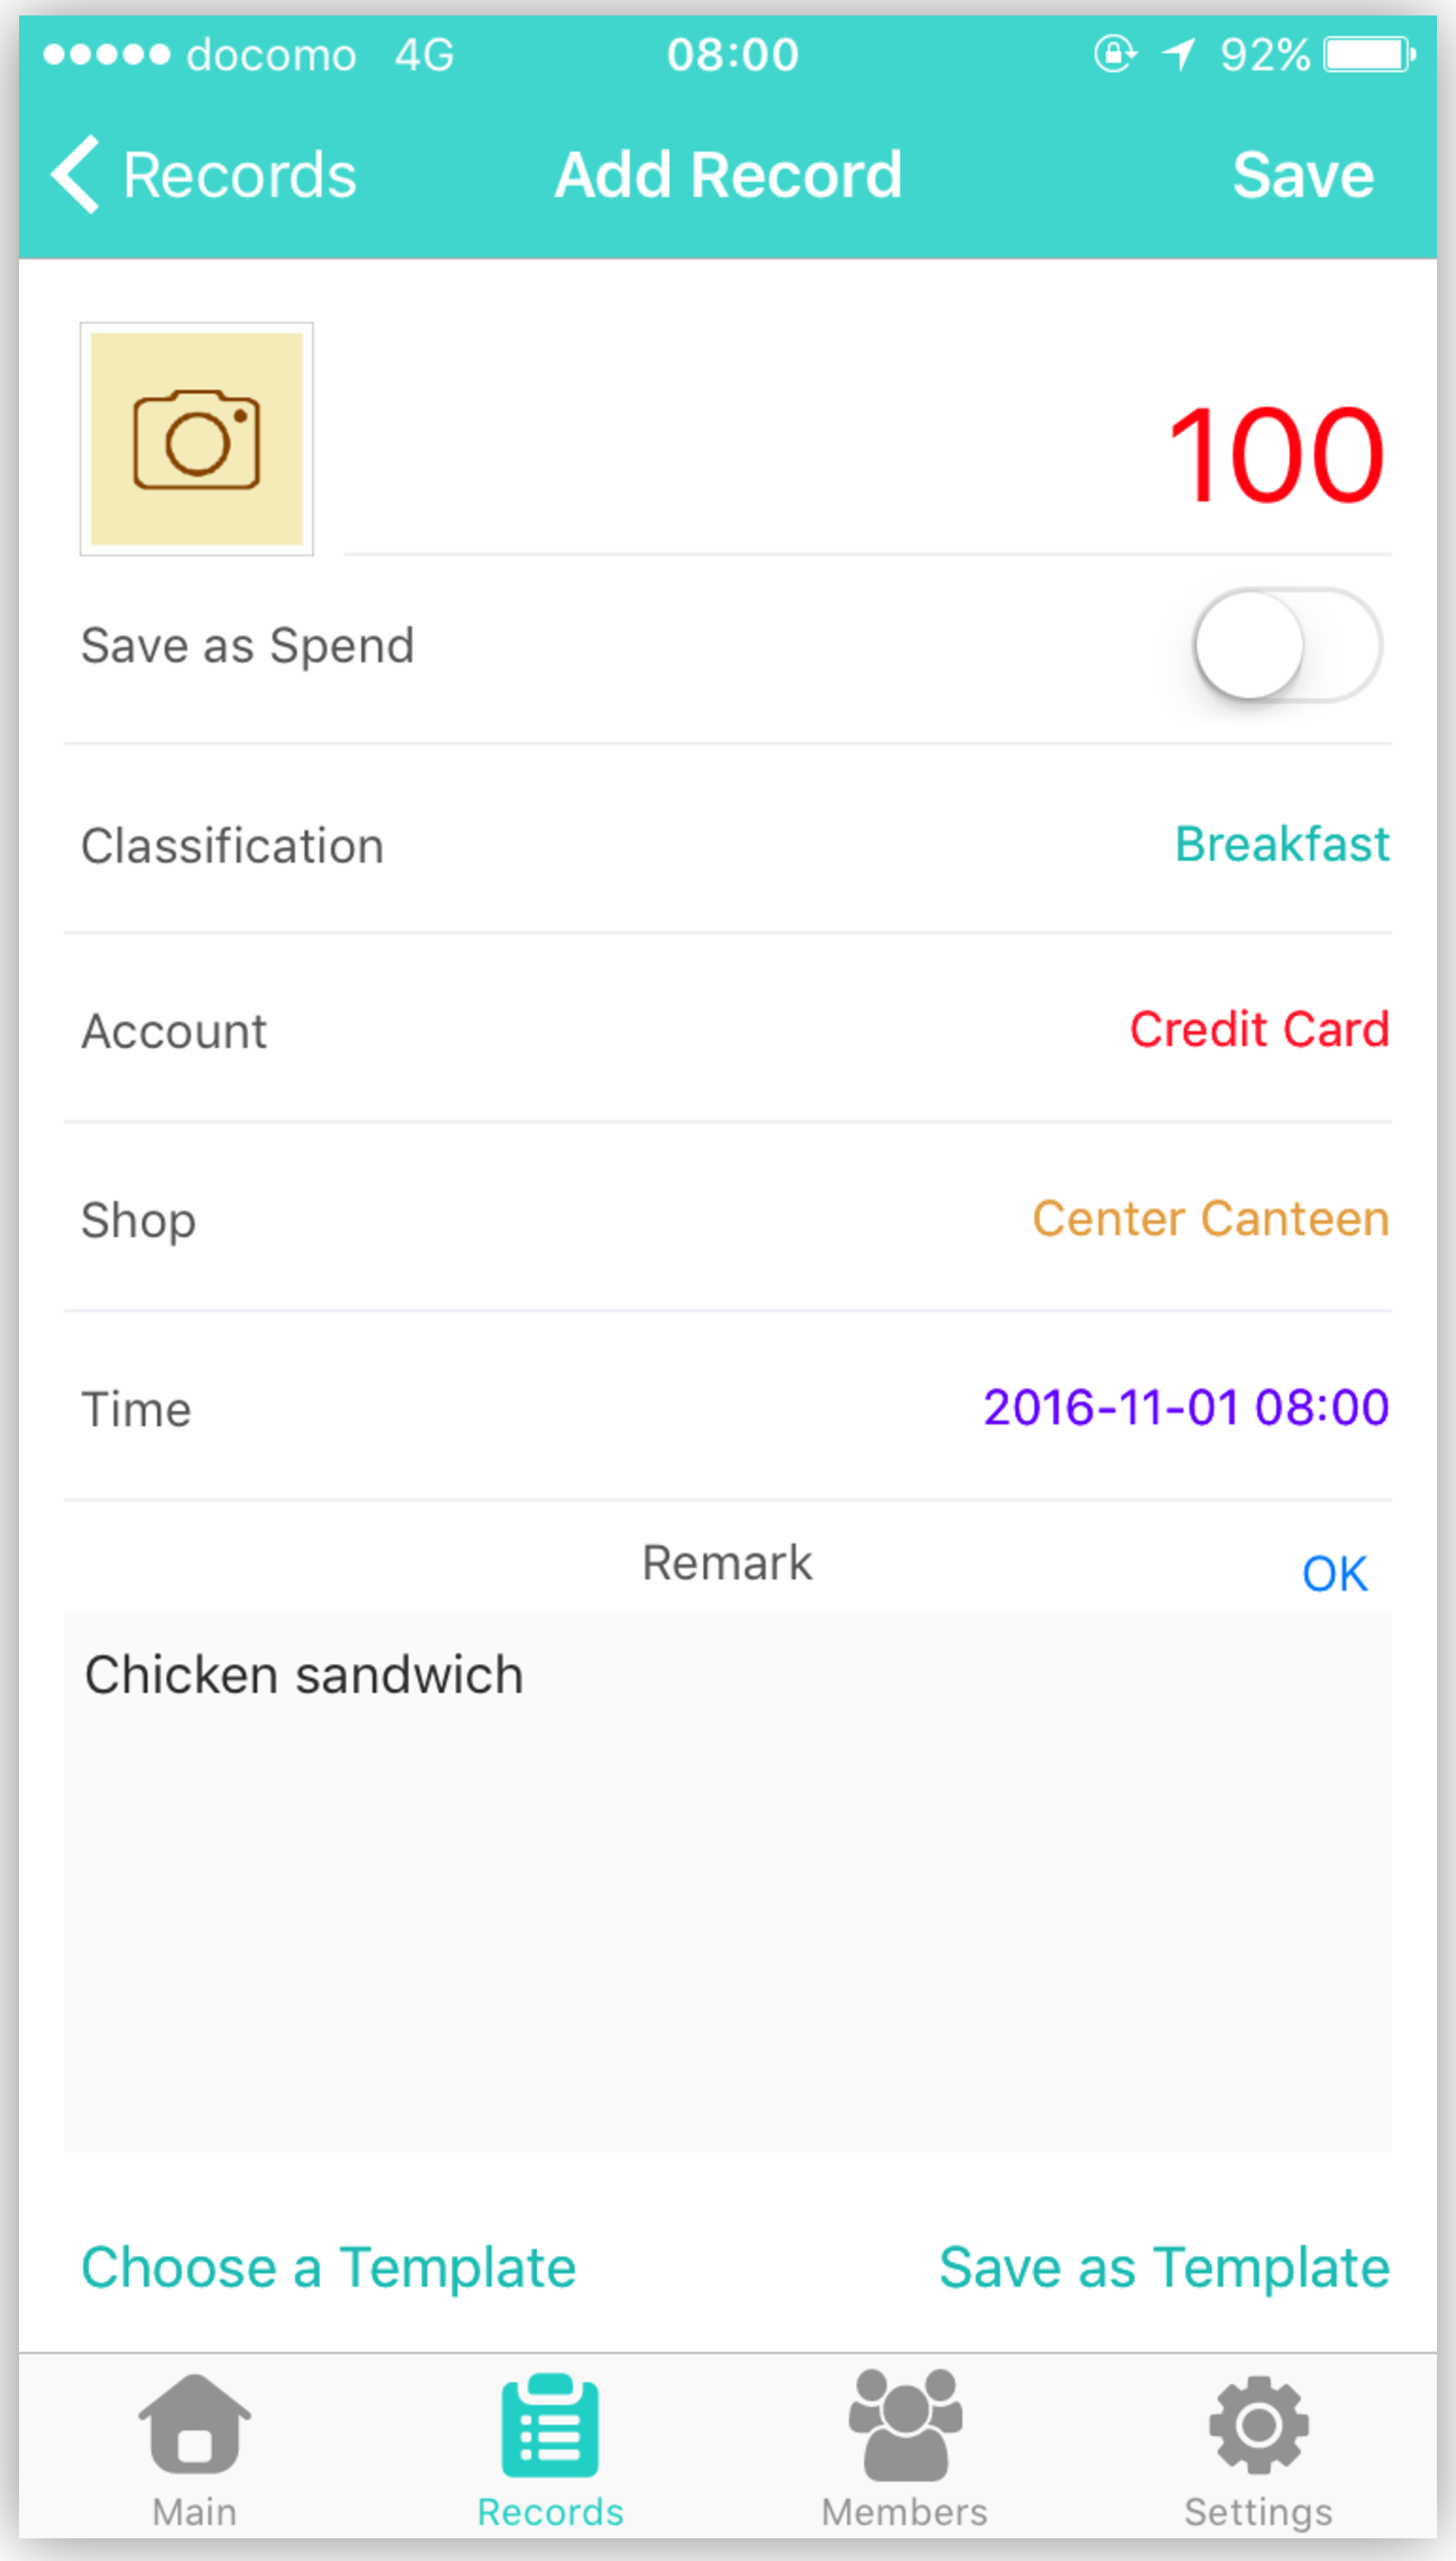
\includegraphics[scale=0.18]{screenshoot}
	\caption{A screen shoot of adding a record.}
\end{figure}

\subsection{Web Service}
Many applications with synchronization use commercial cloud services like Amazon S3, Google Cloud and others. Grouper needs its own Web service rather than using commercial general cloud services for following reasons:

\begin{itemize}
\setlength{\itemsep}{1pt}
\setlength{\parskip}{0pt}
\setlength{\parsep}{0pt}
	\item The Web service supports reliable synchronization.
    \item The Web service ensures that shares are deleted after a prescriptive time.
    \item The Web service allows only group members who have access keys to download shares.
\end{itemize}

Our Web service runs on the Tomcat server that is an open source implementation of the Java Servlet, JavaServer Pages, Java Expression Language and Java WebSocket technologies. We use the Spring Web model-view-controller (MVC) framework to create our REST API. Like in the iOS application, we use Hibernate, an open source Java persistence framework, to save and operate object in the Web service. Hibernate enables developers to easily write applications whose data outlives the processes of the applications.

There are three entities including \emph{Group}, \emph{User} and \emph{Transfer} in our Web service. Figure 6 describes the attributes of these entities and relationship between them. The relationship between \emph{Transfer} and \emph{User} and the relationship between \emph{User} and \emph{Group} are \emph{many-to-one}. The \emph{Group} entity has the unique identifier, group name and its owner. The \emph{User} entity has basic information of a user, access key for this user, and group of this user. The \emph{Transfer} entity has a share generated with a secret sharing scheme, the time when the user uploads it and its creator. For each user, there is a unique access key for him in an untrusted server. Thus, only this user can modify or remove what he uploaded to this server. For a group, one of a user is its owner who has the highest privilege of this group.

\begin{figure}[t]
	\centering
	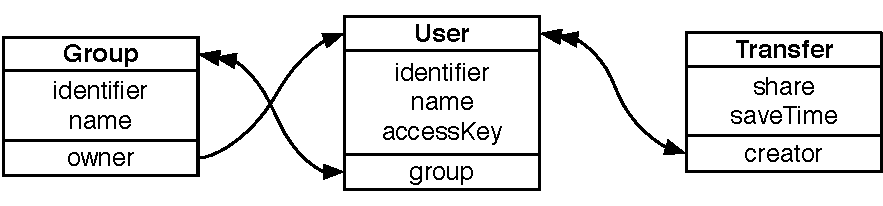
\includegraphics[scale=0.5]{entites}
	\caption{Entities in the Web service.}
\end{figure}

\section{Related Work}

DepSky\cite{bessani2013depsky} is a system that stores encrypted data on servers and runs application logic. DepSky provides a storage service that improves the availability and confidentiality by using commercial storage services. \emph{Cloud-of-Clouds} is the core concept in DepSky. It represents that DepSky is a virtual storage, and its users invoke operations in several individual severs. DepSky keeps encrypted data in commercial storage services and do application logic in individual servers. In Grouper,  untrusted servers undertake responsibility of temporarily data storage and message delivery with server-side computation.

Mylar\cite{popa2014building} stores encrypted and sensitive data on a server, and decrypts this data only in users’ browsers. Developers of Mylar use its API to encrypt a regular(non-encrypted) Web application, and users decrypt data by a browser extension. Like in Grouper, applications in Mylar can control how user data is shared. Mylar builds its system on a browser with extension while Grouper uses mobile devices.

There are many applications and frameworks that use untrusted networks and servers. Compared to them, Grouper uses secret sharing and temporary data storage with untrusted servers to protect user data. Using secret sharing is more convenient and faster than using data encryption because clients need not to distribute decryption keys and perform heavy encryption computation.

\section{Conclusion}

This paper introduces Grouper, a group finance manager that synchronizes data among mobile devices with multiple untrusted servers. Grouper uses secret sharing and temporary data storage services. Grouper consists of clients that run an iOS application and multiple untrusted servers that run a Web service. Each server of Grouper does not know the others and keeps one piece of the shares generated by secret sharing temporarily to protect user data. We connect clients and multiple untrusted servers by a REST API. We are developing a robust protocol of reliable synchronization using multiple untrusted servers.

\bibliographystyle{unsrt}
{
	\footnotesize
	\bibliography{ref}
}

\end{document}
